%Cody Lewis, 2012
%Visit anzhelka.com for all the latest
%
% CTRL+SPACE to switch panes
%


% Note: blank lines indicate a new paragraph
% Note: \left( and \right) cannot break lines.

\documentclass{article}

\usepackage{amsmath}
\usepackage{longtable} %for tables that can break across pages
\usepackage{graphicx}
\usepackage{fancyhdr} % Fancy Header


%\usepackage{hyperref} %Must be at the end of use package but befor "other settings". Used to make links of all references.




\numberwithin{equation}{section} %change the numbering to have something like 1.1 and 3.15, etc.

%Format of macro:la
%\newcommand{\NAME}[ARGUMENT NUMBER (OPTIONAL)]{ stuff to include, arguments denoted #1, #2, etc. }
\newcommand{\vect}[1]{\boldsymbol{#1^2}}
\newcommand{\bigvect}[3]{\boldsymbol{#1^#2^#3}}
\newcommand{\bs}[1]{\boldsymbol{#1}}

\graphicspath{{../figures/}{../extra/}} %\graphicspath{{path/one/}{path/two/}{path/three/}}
\fancyfoot[CO,CE]{ \thepage \\ 
\includegraphics[width=2cm]{../extra/pheonix_small.png}}
\pagestyle{fancy}

\begin{document}

\title{Quadrotor Mathematics For Simpletons}
\author{Cody Lewis \\ \texttt{srlm@anzhelka.com} \and Luke De Ruyter \\ \texttt{ilukester@anzhelka.com} }
\date{\today}
\maketitle
\begin{verse}\textit{
And when he [Herod] had apprehended him [Peter], he put him in prison, and delivered him to four quaternions of soldiers to keep him; intending after Easter to bring him forth to the people.} \\
\hfill --Acts 12:14, King James Bible, Cambridge Edition
\end{verse}

\begin{abstract}
This paper describes in detail the dynamics of a quadrotor platform. Most current research papers simply explain the equations without explaining derivations or reasoning behind the numbers. This paper will explain and derive the equations for a quadrotor aircraft based an the system found in \cite{stingu09}.
\end{abstract}

%% S1 S1 S1 S1 S1 S1 S1 S1 S1 S1 S1 S1 S1 S1 S1 S1 S1 S1 S1 S1  
\section{Introduction}
%% S1 S1 S1 S1 S1 S1 S1 S1 S1 S1 S1 S1 S1 S1 S1 S1 S1 S1 S1 S1  

\begin{figure}[h!]
  \centering
	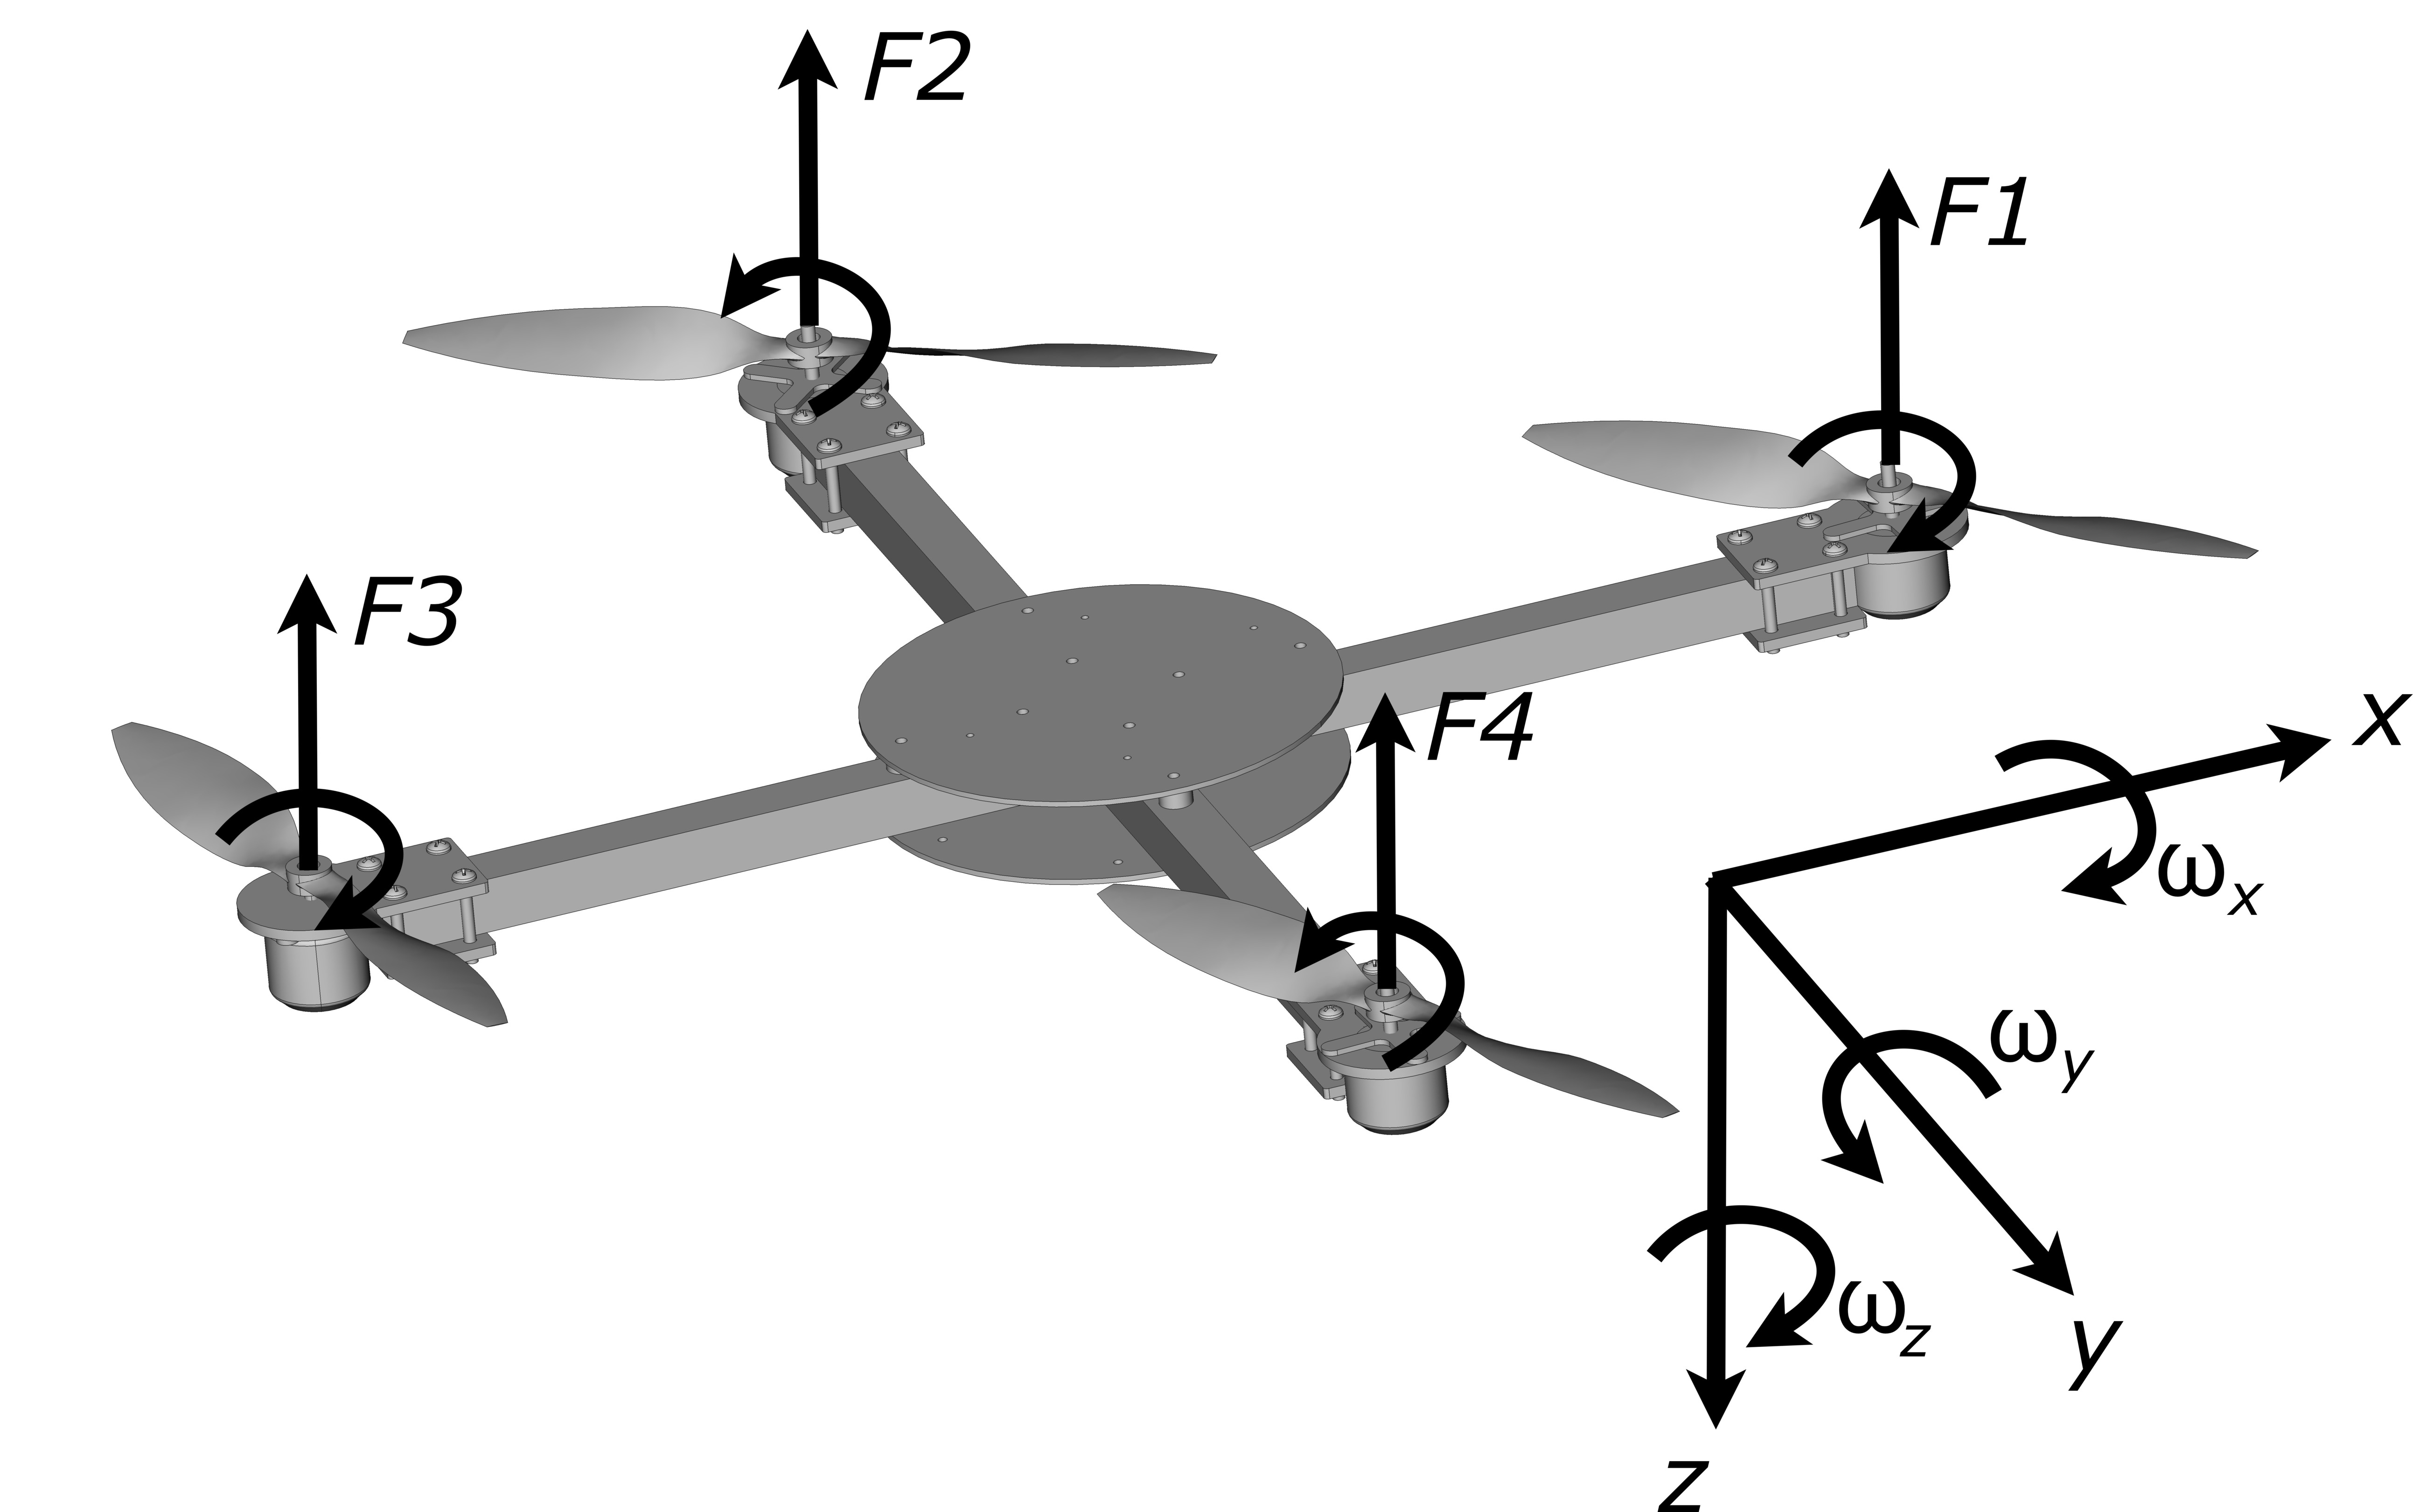
\includegraphics[scale=.05]{reference_frame_diagram.jpg}
  \caption{Orientation of the body axis with respect to the motor numbers and rotations.}
\end{figure}  

A quadrotor is a simple aerial vehicle much like a helicopter, but instead of a single main rotor a quadrotor has four rotors. This allows for a much simpler mechanical system, since each rotor can be directly mounted to it's motor without any linkages to change the pitch of a rotor.

Quadrotor dynamics are very complex. It's difficult because you have four motors, all pointed in the same direction, and that's it. But yet the vehicle can move on three axes in translational motion, and can rotate about another three axes. A quadrotor must be able to convert the four motor inputs into these six different (and often conflicting) motions.

The simplest case is hovering in a single location, and will be dealt with in this paper. Initially it is assumed that the quadrotor will have negligible translational motion in the global x-y plane, although eventually the translational equations may be added to this paper.

The quadrotor used in this paper is assumed to be fairly simple. The platform must be able to measure the following components:
\begin{list}{*}{}
	\item rotation (direction and velocity)
	\item translation (velocity and accleration)
	\item motor rotational speed
	\item air density
\end{list}
Note that if air density is assumed to be constant than performance may suffer at different altitudes or weather. In addition, the following constants must be empirically measured for each quadrotor vehicle:
\begin{list}{*}{}
	\item mass ($kg$)
	\item moment of inertia tensor ($kg \cdot m^2$)
	\item offset of each rotor from the center of mass ($m$)
	\item thrust coefficient (see subsection \ref{subsec:thrustandtorquecoefficientmeasurements})
	\item torque coefficient (see subsection \ref{subsec:thrustandtorquecoefficientmeasurements})
	\item rotor diameter ($m$)
\end{list}

The quadrotor system is complicated by the fact that a quadrotor will need to be able to balance itself in flight. If a gust of wind blows from the side and rolls the quadrotor, it will no longer be in a stable hover. The controller will need to increase the speed of some motors and decrease the speed of others so that the vehicle is rotated back into a vertical hovering state.

There is still a problem: each motor is producing torque on the body as well as thrust. This is manifested by the motor "attempting" to rotate the body due to the spinning mass of the motor and propeller, and the air resistance the propeller encounters. On a quadrotor frame we have two motors spinning clockwise and two spinning counter clockwise, and the torques cancel each other out. But if a motor's speed in increased to account for a tilt, then it's torque on the frame will increase as well, causing the whole body to rotate.

And so now, when a gust of wind blows on the frame, we have to somehow correct the tilt without allowing the torque to yaw the frame. At other times we may want to yaw without tilting, and sometimes we want to do both simultaneously.  There is so much more beyond just the basic thrust, tilt, and yaw: we have to account for many factors such as free stream velocity (or air, in layman's terms) through the propellers, blade flapping, sensor failure, and the many small equations required to support the main equations.

%% S1 S1 S1 S1 S1 S1 S1 S1 S1 S1 S1 S1 S1 S1 S1 S1 S1 S1 S1 S1  
\section{Symbols Used}
%% S1 S1 S1 S1 S1 S1 S1 S1 S1 S1 S1 S1 S1 S1 S1 S1 S1 S1 S1 S1  

%% S2 S2 S2 S2 S2 S2 S2 S2 S2 S2 S2 S2 S2 S2 S2 S2 S2 S2 S2 S2  
\subsection{Variables}
%% S2 S2 S2 S2 S2 S2 S2 S2 S2 S2 S2 S2 S2 S2 S2 S2 S2 S2 S2 S2  

Variables with the subscript $i$ denote association with motor $i$.\\
\begin{longtable}{p{2cm}p{8cm}}
 	$ \bs{\omega}_{b} $ 	& angular velocity in the body frame ($rad/s$) \\
 	$ \mathbf{q} $ 			& attitude quaternion \\
 	$ \tilde{\mathbf{q}} $	& error quaternion \\
 	$ \mathbf{q}_d $		& desired quaternion \\
 	$ \boldsymbol{V}_{b} $ 	& velocity in the body frame ($m/s$) \\
 	$ \boldsymbol{R}_{e} $	& position in the inertial frame ($m$) \\
 	$ F_{z} $				& total force of the rotors on the z axis ($N$) \\
 	$ M_{x} - M_{z} $		& total rotor moments along each axis ($N \cdot m$) \\
 	$ F_{1} - F_{4} $		& thrust force of each rotor ($N$) \\
 	$ Q $					& rotor torque ($N \cdot m$) \\
 	$ T $					& rotor thrust force ($N$) \\
 	$ n_i $					& rotation frequency of the rotors ($Hz$) \\
 	$ \Omega_i $			& rotation speed of the rotors ($rad / s$) \\	
 	$ \Omega_{di} $			& desired rotation speed of the rotors ($rad / s$) \\
 	$ \Omega_{imeas} $		& measured rotation speed of the rotors ($rad / s$) \\
 	$ \hat{\Omega}_i $		& expected speed ($rad / s$) \\
 	$ u_i $					& motor command ($???$) \\
 	$ a_i $					& motor gain (no units) \\
 	$ \psi $				& yaw angle ($???$) \\
 	$ \gamma_H $			& tilt direction in the x-y plane ($???$) \\
 	$ \alpha_H $			& tilt amount around $\gamma_H$ ($???$) \\
 	$ \bs{q}_V$				& yaw error \\
 	$ \bs{q}_H$				& tilt error \\
 	$ \begin{bmatrix}
 		r_x \\
 		r_y \end{bmatrix}$	& tilt axis in the $x-y$ plane ($???$) \\
 	$ \beta_H $				& direction of the tilt axis in the $x-y$ plane ($???$) \\
	$ K_{tilt} $			& amount of tilt in the system? (from altitude controller) \\
	 	
\end{longtable}

%% S2 S2 S2 S2 S2 S2 S2 S2 S2 S2 S2 S2 S2 S2 S2 S2 S2 S2 S2 S2  
\subsection{Constants}
%% S2 S2 S2 S2 S2 S2 S2 S2 S2 S2 S2 S2 S2 S2 S2 S2 S2 S2 S2 S2  

\begin{longtable}{p{2cm}p{8cm}}
 	$ \bs{I}_{nb} $			& moment of inertia tensor ($kg \cdot m^{2}$) \\
 	$ D $ 					& rotor diameter ($m$) \\
 	$ d $					& offset of each rotor from the center of mass ($m$) \\
 	$ \rho $				& air density ($kg/m^3$) \\
 	$ K_t $					& thrust coefficient ($???$) \\
 	$ K_q $					& torque coefficient ($???$) \\
 	$ K_g $					& the speed adaptable gain for $a_i$ ($???$) \\
 	$ f_{mot}( \cdot ) $	& motor response function ($???$) \\
 	$ \tau $				& time constant, step ($???$) \\
 	$K_{PH} $				& tilt moment proportional constant \\
 	$K_{DH} $				& tilt moment derivative constant \\
 	$K_{Pz} $				& yaw moment proportional constant \\
 	$K_{Dz} $				& yaw moment derivative constant \\
 	$F_{PIDz} $				& proportional altitude controller ($N$ ?) \\
 	$m$						& quadrotor mass ($kg$ ?) \\
 	$g$						& local gravity ($m/s^2$) \\
 	$K_{P_z}$				& Proportional PID gain for $F_z$ \\
	$K_{I_z}$				& Integral PID gain for $F_z$ \\
	$K_{I_z}$				& Derivative PID gain for $F_z$ \\
 	$ K_{P_i} $				& Motor Proportional PID gain (for $1 \leq i \leq 4$) \\
 	$ K_{I_i} $				& Motor Integral PID gain (for $1 \leq i \leq 4$) \\
 	
\end{longtable}

%% S1 S1 S1 S1 S1 S1 S1 S1 S1 S1 S1 S1 S1 S1 S1 S1 S1 S1 S1 S1  
\section{Introduction to Quaternions}
%% S1 S1 S1 S1 S1 S1 S1 S1 S1 S1 S1 S1 S1 S1 S1 S1 S1 S1 S1 S1  
This paper represents orientation using quaternions. There are other methods of representing rotation, but a quaternion has several advantages that lend it well to use on the quadrotor:
\begin{list}{*}{}
	\item Quaternions avoid gimbal lock (where two rotation axes align on each other during the course of a rotation, producing unnatural results)
	\item Quaternions have smaller memory requirements (4 floats) than other representations
	\item Quaternions have much more efficient mathematical operations, and don't require orthonormalization (making the axes orthogonal after an imprecise computation) like a rotation matrix does.
	\item Quaternions allow for smooth interpolation between two orientations.
	\item Orientation updates (updating a refernce orientation with $\omega$, for example) do not require trigonometric functions.
\end{list}

A quaternion is a way of representing a rotation. This is similar to Euler angles, but has the advantage of a more concise notation (and math), and not having singularities like Euler angles have. Quaternions are difficult to visualize from the numbers, but are easy enough to understand and use.

A quaternion is geometrically defined as follows:

$$ \boldsymbol{q} = 
	\left[ 
		\begin{array}{c}
			q_0 \\
			q_1 \\
			q_2 \\
			q_3 \\
		\end{array}
	\right]	
	=	
	\left[
		\begin{array}{c}
			\cos \left( \alpha / 2 \right) \\
			\sin \left( \alpha / 2 \right) \cdot \boldsymbol{r}
		\end{array}
	\right]	
$$

This means that the rotation is around the axis $\boldsymbol{r}$ and by amount $\alpha$. Note that in the second representation the second element is $q_1$, $q_2$, and $q_3$ (it's three because of the $\cdot \boldsymbol{r}$, which is a three element vector). To add some terminology, the first term $q_0$ is called the scalar part, while $q_1$ through $q_3$ is called the vector part.

A quaternion can be thought of a number, just like any other. So, we can do several operations such as add, multiply, invert (divide), take the norm, and of course test for equality. We'll be focusing on rotation quaternions for the rest of this paper. A rotation quaternion is the specific form of quaternion used to represent rotation, and must have a norm equal to one. It should be noted here that a rotation quaternion is of length one (unit) only by convention and because it simplifies some proofs, but that any non-zero real multiple of $q$ gives the the same rotation (although the interpretation of rotating by $\Omega$ about $v$ is lost for non-unit quaternions).

We define the norm of quaternion as

$$ \lVert q \rVert = \sqrt{q_0^2 + q_1^2 + q_2^2 + q_3^2} $$

The norm can be thought of as the "length" of a quaternion (or vector, etc). A $ \lVert q \rVert $ value of 1 is called a unit quaternion. In quaternion literature there seems to be a discrepancy: some authors define the quaternion norm as above, with a square root, while others omit the square root (e.g. \cite{shoemake69}). In this paper we will use the norm with a square root. This is called the L2-norm, or more commonly the Euclidean norm. I couldn't find anything on a norm that squared it's components but had no root, so we'll ignore it (for more information on norms, see \cite{malek09}).

We also define the conjugate and inverse of a rotation quaternion as

$$ q^* = q' = \left(q_0, -q_1, -q_2, -q_3 \right) = q^{-1} $$

Note this equality is only true for unit quaternions (rotation quaternions), and does not hold for other quaternions.

The only binary operation that we will be using for rotation quaternions is multiplication, denoted by $ \otimes$. Note that quaternion multiplication is not commutative. Multiplying $q_1 \otimes q_2 \neq q_2 \otimes q_1 $. Multiplying rotation quaternions produces a third rotation quaternion that is the result of rotating each quaternion in reverse order starting with the right hand side quaternion. To rotate a standard vector from one coordinate system to another simply place it into the vector part of the quaternion and set the scalar part to zero. Then, for transforming the vector $r_e$ to the vector $r_b$:

\begin{align}
	\begin{bmatrix}
		0 \\
		r_b \\
	\end{bmatrix}
	&=
	\bs{q}^* \otimes 
	\begin{bmatrix}
		0 \\
		r_e \\
	\end{bmatrix}
	\otimes \bs{q}	\\
	\begin{bmatrix}
		0 \\
		r_e \\
	\end{bmatrix}
	&=
	\bs{q} \otimes 
	\begin{bmatrix}
		0 \\
		r_b \\
	\end{bmatrix}
	\otimes \bs{q}^*	\\	
\end{align}	
		
For the rest of this paper, if a vector is rotated by a quaternion it will  be written as a vector but assumed to be in the vector part of a quaternion. For example,

\begin{equation}
	\omega_b' = \bs{q} \otimes \omega_b, \qquad 	\textrm{where} \quad
	\omega_b =	
	\begin{bmatrix}
		0 \\
		\omega_b \\
	\end{bmatrix}
\end{equation}
The vector $\omega_b$ is rotated by quaternion $\bs{q}$ to get the rotated vector $\omega_b'$.

The product of two quaternions is another quaternion and is defined as:
\begin{equation}
	\begin{split}
		%Note that \left( and \right) did not seem to work...
		p \otimes q =	( & p_0 q_0 - p_1 q_1 - p_2 q_2 - p_3 q_3, \\
							& p_0 q_1 + p_1 q_0 + p_2 q_3 - p_3 q_2,  \\
							& p_0 q_2 + p_2 q_0 + p_3 q_1 - p_1 q_3,  \\
							& p_0 q_3 + p_3 q_0 + p_1 q_2 - p_2 q_1 ) \\
	\end{split}
\end{equation}

One thing to note is that a quaternion multiplication has 12 scalar additions and 16 scalar multiplies. Since the components are floating point numbers, each quaternion multiplication consumes 28 floating point operations. \\

%% S1 S1 S1 S1 S1 S1 S1 S1 S1 S1 S1 S1 S1 S1 S1 S1 S1 S1 S1 S1  
\section{Basic Equations}
%% S1 S1 S1 S1 S1 S1 S1 S1 S1 S1 S1 S1 S1 S1 S1 S1 S1 S1 S1 S1
In this section we will cover in detail all of the equations necessary to fly. This section explains the derivation and reasoning behind each equation used, and any assumptions that are made.
%% S2 S2 S2 S2 S2 S2 S2 S2 S2 S2 S2 S2 S2 S2 S2 S2 S2 S2 S2 S2  
\subsection{Roll, Pitch, and Yaw Errors} \label{subsec:rollpitchyawerrors}
%% S2 S2 S2 S2 S2 S2 S2 S2 S2 S2 S2 S2 S2 S2 S2 S2 S2 S2 S2 S2  

The control of a quadrotor must first consider maintaining a desired attitude. For hover, the attitude would be with no roll or pitch, and possibly some yaw. We start by generating a desired orientation $\bs{q}_d$. This can be either a from some software routine (autonomous), or perhaps from a user control (ie, the orientation of a control board). Given the current orientation $\bs{q}$, the quadrotor must be turned through some rotation $\tilde{\bs{q}}$. Hence,
\begin{eqnarray}
\bs{q}_d = \tilde{\bs{q}} \otimes \bs{q} \\
\tilde{\bs{q}} = \bs{q}_d \otimes \bs{q}^* \label{eq:errorquaternion}
\end{eqnarray}
Rewritten using the geometric definition of a quaternion,
\begin{equation} \label{eq:errorquaternion_geometric}
\tilde{\bs{q}} = 
	\begin{bmatrix}
		\cos \left( \alpha / 2 \right) \\
		\sin \left( \alpha / 2 \right) \cdot \bs{r}_e
	\end{bmatrix}
\end{equation}
Equation \eqref{eq:errorquaternion_geometric} says that the error quaternion is composed of an angle $\alpha$ and a vector $\bs{r}_e$ (remember, the e subscript denotes the earth reference frame). From equation \eqref{eq:errorquaternion} we have the value of $\tilde{\bs{q}}$, so equation \eqref{eq:errorquaternion_geometric} should be rewritten as
\begin{equation}
\begin{bmatrix}
	\cos \left( \alpha / 2 \right) \\
	\sin \left( \alpha / 2 \right) \cdot \bs{r}_{e_1} \\
	\sin \left( \alpha / 2 \right) \cdot \bs{r}_{e_2} \\
	\sin \left( \alpha / 2 \right) \cdot \bs{r}_{e_3} \\
\end{bmatrix}
=
	\begin{bmatrix}
		\tilde{q_0} \\
		\tilde{q_1} \\
		\tilde{q_2} \\
		\tilde{q_3} \\
	\end{bmatrix}
\end{equation}
This puts the four known $\tilde{q_i}$ on the right hand side and the unknown $\alpha$ and three $\bs{r}_{e_j}$ on the left hand side. Solving, we have
\begin{equation} \label{eq:errorquaternionalpha}
\alpha = 2\arccos{\left(\tilde{q_0}\right)}
\end{equation}
And, using the calculated $\alpha$ we solve the following:
\begin{eqnarray}
\bs{r}_{e_1} = \frac{\tilde{q_1}}{\sin{\alpha/2}} \\
\bs{r}_{e_2} = \frac{\tilde{q_2}}{\sin{\alpha/2}} \\
\bs{r}_{e_3} = \frac{\tilde{q_3}}{\sin{\alpha/2}} \\
\end{eqnarray}
The vector $\bs{r}_e$ is in earth coordinates, so using the properties of quaternion rotation we must rotate it into body coordinates to determine which movements are necessary.

%Question: should $\alpha$ in the equations above and below have the subscript $\alpha_h$ like later in this section? ---A: No, because the above alpha is the rotation for the error quaternion, and the alpha_h is the alpha for the q_h quaternion

\begin{equation} 
\bs{r}_b = \bs{q}^* \otimes \bs{r}_e \otimes \bs{q}
\end{equation}
And now we can create the error quaternion in body coordinates $\tilde{\bs{q}}_b$. Note that $\alpha$ is the same as in equation \eqref{eq:errorquaternionalpha}. Even though the two vectors $\bs{r}_e$ and $\bs{r}_b$ differ numerically, they are really identical except for being in different coordinate systems. So the rotation $\alpha$ is the same.
\begin{equation} \label{eq:qberror}
\tilde{\bs{q}}_b = 
\begin{bmatrix}
	\cos \left( \alpha / 2 \right) \\
	\sin \left( \alpha / 2 \right) \cdot \bs{r}_b
\end{bmatrix}
\end{equation}
Instead of defining three different angles of rotation (ie, roll, pitch, and yaw) this paper will define the body rotation as tilt (encompassing both roll and pitch) and yaw. This can be written as
\begin{equation} \label{eq:errorquaternionyawtilt}
\tilde{\bs{q}}_b = \bs{q}_H \otimes \bs{q}_V
\end{equation}
where $\bs{q}_H$ is the tilt error and $\bs{q}_V$ is the yaw error. From the definition of the quaternion, we can rewrite \eqref{eq:errorquaternionyawtilt} in the geometric form and expand the quaternion multiplication.

\begin{align}
	\begin{bmatrix}
		q_0 \\
		q_1 \\
		q_2 \\
		q_3 \\
	\end{bmatrix}
	&=
	\begin{bmatrix}
		\cos \left( \alpha_H / 2 \right) \\
		\sin \left( \alpha_H / 2 \right) \cdot r_x \\
		\sin \left( \alpha_H / 2 \right) \cdot r_y \\
		\sin \left( \alpha_H / 2 \right) \cdot 0 \\
	\end{bmatrix}
	\otimes
	\begin{bmatrix}
		\cos \left( \psi / 2 \right) \\
		\sin \left( \psi / 2 \right) \cdot 0 \\
		\sin \left( \psi / 2 \right) \cdot 0 \\
		\sin \left( \psi / 2 \right) \cdot 1 \\
	\end{bmatrix} \notag \\
	&=
	\begin{bmatrix}
		\cos \left( \alpha_H / 2 \right) \\
		\sin \left( \alpha_H / 2 \right) \cdot r_x \\
		\sin \left( \alpha_H / 2 \right) \cdot r_y \\
		0 \\%\sin \left( \alpha_H / 2 \right) \cdot 0 \\
	\end{bmatrix}
	\otimes
	\begin{bmatrix}
		\cos \left( \psi / 2 \right) \\
		0 \\ %\sin \left( \psi / 2 \right) \cdot 0 \\
		0 \\ %\sin \left( \psi / 2 \right) \cdot 0 \\
		\sin \left( \psi / 2 \right) \cdot 1 \\
	\end{bmatrix} \notag \\
	&=
	\begin{bmatrix}
		\cos \left( \alpha_H / 2 \right) \cos \left( \psi / 2 \right) - 0 - 0 - 0 \\
		0 + \sin \left( \alpha_H / 2 \right) \cdot r_x \cos \left( \psi / 2 \right)  + \sin \left( \alpha_H / 2 \right) \cdot r_y \sin \left( \psi / 2 \right) + 0 \\
		0 + \sin \left( \alpha_H / 2 \right) \cdot r_y \cos \left( \psi / 2 \right) + 0 - \sin \left( \alpha_H / 2 \right) \cdot r_x \sin \left( \psi / 2 \right) \\
		\cos \left( \alpha_H / 2 \right) \sin \left( \psi / 2 \right)  + 0 + 0 + 0 \\
	\end{bmatrix}
\end{align}
$\alpha_H$ is the amount of tilt, positive by convention (note it is not the same as $\alpha$ in \ref{eq:qberror} and earlier equations). $r_x$ and $r_y$ is the tilt axis in the body $x-y$ plane, and $\psi$ is the yaw angle. Next, using simple algebra we can solve for the four unknowns ($\alpha_H$, $\psi$, $r_x$, and $r_y$) with the four knowns ($q_i$). This gives the following four results:

\begin{align}
	\alpha_H &= \arccos \left[1 - 2 \left( q_1^2 + q_2^2 \right) \right]	&0 \leq \alpha_H < \pi \\
	\psi &= 2 \arctan_2 \left( q_3, q_0 \right) &-\pi \leq \psi < \pi \\
	r_x &=   \frac{\cos \left( \psi / 2 \right) q_1 - \sin \left( \psi / 2 \right) q_2}
	{ \sin \left( \alpha_H / 2 \right) } &\\
	r_y &=   \frac{\sin \left( \psi / 2 \right) q_1 - \cos \left( \psi / 2 \right) q_2}
	{ \sin \left( \alpha_H / 2 \right) } &
\end{align}

We can now find the direction of the tilt axis $\beta_H$:
\begin{equation}
	\beta_H = \arctan_2 \left(r_y, r_x \right)
\end{equation}

With $\alpha_H$, $\psi$, and $\beta_H$ we are now have enough information to stabilize the quadrotor platform. We now turn in the next section to creating a PID control.

%\begin{equation}
%	\gamma_H = \arctan_2 \left(r_x, r_y \right)
%\end{equation}

%Question: are $\beta_H$ and $\gamma_H$ perpendicular or somehow constant relative to one another? ---A: Yes, they are 90 perpendicular.

%% S2 S2 S2 S2 S2 S2 S2 S2 S2 S2 S2 S2 S2 S2 S2 S2 S2 S2 S2 S2  
\subsection{Attitude Stabilization} \label{subsec:attitudestabilization}
%% S2 S2 S2 S2 S2 S2 S2 S2 S2 S2 S2 S2 S2 S2 S2 S2 S2 S2 S2 S2  

Attitude is controlled via a very simple PID loop. The main thing to note here is the use of $\beta_H$ to weight the $\alpha_H$ term to the correct axes. The $\omega$ terms (angular rate) can be measured directly from onboard gyroscopes.

\begin{align}
	M_x &= K_{PH} \alpha_H \cos \beta_H - K_{DH} \omega_x \\
	M_y &= K_{PH} \alpha_H \sin \beta_H - K_{DH} \omega_y \\
	M_z &= K_{Pz} \psi - K_{Dz} \omega_z \\
\end{align}



%% S2 S2 S2 S2 S2 S2 S2 S2 S2 S2 S2 S2 S2 S2 S2 S2 S2 S2 S2 S2  
\subsection{Altitude Stabilization} \label{subsec:altitudestabilization}
%% S2 S2 S2 S2 S2 S2 S2 S2 S2 S2 S2 S2 S2 S2 S2 S2 S2 S2 S2 S2  
The current altitude can be measured in any number of ways. Many quadrotors use an ultrasonic sensor mounted on the bottom of the platform to measure distance to the ground. Alternatively, a system could use an IR sensor, altimeter module, precision differential GPS, or any system that gives a single scalar number as the altitude. This section assumes that whatever measurement was used, the current altitude can be represented a scalar number.
\\ \\
To stabilize the altitude, we define the altitude error as
\begin{equation}
\tilde{\bs{R}}_{e_z} = \bs{R}_{e_z} - desired \left( \bs{R}_{e_z} \right)
\end{equation}
Then we have a simple PID equation for the altitude:
\begin{equation} \label{eq:altitudePID}
	F_{PIDz} = K_{Pz} \tilde{\bs{R}}_{e_z} + K_{Iz} \Sigma \tilde{\bs{R}}_{e_z} + K_{Dz} \dot{\tilde{\bs{R}}}_{e_z}
\end{equation}
In order to obtain the final force along the body $z$ axis, equation \eqref{eq:altitudePID} must be augmented with information about the weight of the quadrotor and the angle the quadrotor is tilted at:
\begin{equation}
	F_z = \frac{mg + F_{PIDz}} {K_{tilt}}
\end{equation}
\begin{equation}
	K_{tilt} = 
	\begin{bmatrix}
		0 & 0 & 1 \\	
	\end{bmatrix}
	\cdot
	\left(
		q \otimes
			\begin{bmatrix}
				0 \\
				0 \\
				-1 \\
			\end{bmatrix}
		\otimes q^*
	\right)
\end{equation}
With these equations, the more the body is tilted the $F_z$ will become and the faster the quadrotor will move in the $x-y$ plane, without a mathematical bound. In reality, at some point the motors will become saturated (running at maximum speed) and the quadrotor will not be able to simultaneously maintain a commanded altitude and attitude.




%% S2 S2 S2 S2 S2 S2 S2 S2 S2 S2 S2 S2 S2 S2 S2 S2 S2 S2 S2 S2  
\subsection{Forces to Motor Speeds} \label{subsec:forcestomotorspeeds}
%% S2 S2 S2 S2 S2 S2 S2 S2 S2 S2 S2 S2 S2 S2 S2 S2 S2 S2 S2 S2 
In previous sections we have calculated the desired moments $M_x$, $M_y$, and $M_z$, and the desired force $F_z$. In this section we will take those moments and convert it to the desired rotation speed of each motor.
\\ \\
First, in equation \eqref{eq:rpm_to_Omega} we have a standard conversion from rotational frequency to angular frequency .
 
\begin{equation} \label{eq:rpm_to_Omega}
\Omega_i = 2 \pi n_i
\end{equation}
\\ \\
Each motor generates a thrust in the direction of the motor shaft axis, and a torque around the motor shaft axis. The calculation of $K_T$ and $K_Q$ is discussed in subsection \ref{subsec:thrustandtorquecoefficientmeasurements}.


\begin{equation} \label{eq:motor_thrust}
T = K_T\rho n^2 D^4
\end{equation}

\begin{equation} \label{eq:motor_torque}
Q = K_Q\rho n^2 D^5
\end{equation}

%\begin{equation} \label{eq:motor_thrust}
%K_T = \frac{T}{\rho n^2 D^4}
%\end{equation}
%
%\begin{equation} \label{eq:motor_torque}
%K_Q = \frac{Q}{\rho n^2 D^5}
%\end{equation}

These two equations are used to define $T$ and $Q$. The constants $K_T$ and $K_Q$ are determined experimentally. A motor test stand must be able to measure $T$, $Q$, $\rho$, $n$, and $D$, and generate the constants for a particular motor and propeller combination. Note the exponents in the equations: rotational speed and propeller diameter have a significant effect on the thrust and torque.
\\ \\
For use onboard the quadrotor, equation \eqref{eq:motor_thrust} will be used with equation \eqref{eq:rpm_to_Omega} to connect thrust to rotational speed. This derivation is done in equation \eqref{eq:thrust_to_Omega}. By this combination we will be able to determine what rotational speed we need to run the motors at to achieve a specified thrust. From equations \eqref{eq:motor_thrust} and \eqref{eq:rpm_to_Omega} we rewrite and combine:
\begin{align}
	n^2 	&= \frac{T}{\rho K_T D^4} \notag \\
	n		&= \frac{1}{D^2} \sqrt{\frac{T}{\rho K_T}} \notag \\
	\Omega_{di}	&= 2 \pi n \notag \\	
	\Omega_{di}	&= \frac{2 \pi}{D^2} \sqrt{\frac{T}{\rho K_T}} \label{eq:thrust_to_Omega}
\end{align}
\\ \\
With equation \eqref{eq:thrust_to_Omega} we have an equation that will tie the thrust required to how fast the rotors must spin. This can later be fed into a PI controller for each motor, described in section \ref{subsec:motorcontrol} .
\\ \\
Finally, we need to determine what the thrust and torque of each motor for the given $M$ and $F_z$:

\begin{align}
\begin{bmatrix}
	F_z \\
	M_x \\
	M_y \\
	M_z \\
\end{bmatrix}
&=
\begin{bmatrix}
	1 & 1 & 1 & 1 \\
	0 &-d & 0 & d \\
   -d & 0 & d & 0 \\
	c &-c & c &-c \\
\end{bmatrix}
\cdot
\begin{bmatrix}
	F_1 \\
	F_2 \\
	F_3 \\
	F_4 \\
\end{bmatrix}
\\
\begin{bmatrix}
	1 & 1 & 1 & 1 \\
	0 &-d & 0 & d \\
   -d & 0 & d & 0 \\
	c &-c & c &-c \\
\end{bmatrix}^{-1}
\cdot
\begin{bmatrix}
	F_z \\
	M_x \\
	M_y \\
	M_z \\
\end{bmatrix}
&=
\begin{bmatrix}
	F_1 \\
	F_2 \\
	F_3 \\
	F_4 \\
\end{bmatrix}
\\
%\begin{bmatrix}
%	F_1 \\
%	F_2 \\
%	F_3 \\
%	F_4 \\
%\end{bmatrix}
%&=
%\begin{bmatrix}
\end{align}
where
\begin{equation}
c = \frac{K_Q D}{K_T}
\end{equation}
\\
Solving the matrix inversion and multiplication, we arrive at the final four equations:
\begin{align}
F_1 &= +\frac{M_z}{4c} - \frac{M_y}{2d} + \frac{F_z}{4} \\
F_2 &= -\frac{M_z}{4c} - \frac{M_x}{2d} + \frac{F_z}{4} \\
F_3 &= +\frac{M_z}{4c} + \frac{M_y}{2d} + \frac{F_z}{4} \\
F_4 &= -\frac{M_z}{4c} + \frac{M_x}{2d} + \frac{F_z}{4} \\
%\end{bmatrix}
\end{align}
Now, we have the force (thrust) that each motor must produce in order to maintain the desired heading, and can use equation \eqref{eq:thrust_to_Omega} to determine the desired rotor speed.


%% S2 S2 S2 S2 S2 S2 S2 S2 S2 S2 S2 S2 S2 S2 S2 S2 S2 S2 S2 S2  
\subsection{Motor control} \label{subsec:motorcontrol}
%% S2 S2 S2 S2 S2 S2 S2 S2 S2 S2 S2 S2 S2 S2 S2 S2 S2 S2 S2 S2  

This subsection describes the equations used to set the rotational speed of the motors. Note that this differs from \cite{stingu09}: in that paper the authors used an empirically measured function ($f_{mot}$) to estimate the rotational speed based on the voltage of the motor and the command given. This required a dynamically adjustable constant $a_i$ to calibrate each motor for small differences in manufacturing. In this paper it is assumed that actual motor rotational speed is able to be measured. By measuring the rotational speed of the motors we are able to ignore the manufacturing differences between motors, and create a closed loop control. If a motor is not spinning at the correct speed the PI control loop described next will be able to correct until the desired rotation is achieved.
\\ \\
The following two equations are explicitly defined a discrete time $t$. For clarity, the subscript $i$ denoting a specific motor is implied but not written:
\begin{equation}
	\Omega \left(t \right)_{ Ierror} = \Omega \left(t-1 \right)_{ Ierror} + \left( \Omega_{d} - \Omega_i \right)
\end{equation}
\begin{equation}
	u_i = K_{P} \left( \Omega_{d} - \Omega_i \right) + K_{I} \Omega \left(t \right) _{Ierror}
\end{equation}


%% S2 S2 S2 S2 S2 S2 S2 S2 S2 S2 S2 S2 S2 S2 S2 S2 S2 S2 S2 S2  
\subsection{Quadrotor Motion Model}
%% S2 S2 S2 S2 S2 S2 S2 S2 S2 S2 S2 S2 S2 S2 S2 S2 S2 S2 S2 S2  
The equations in this section describe the motion of the quadrotor body through space. In essence, these equations are taken directly from any introductory physics textbook and simply expanded a small amount. These equations are necessary for translational motion, but are not required to simply hover

\begin{equation} \label{eq:body_acceleration}
\dot{\boldsymbol{V}}_b = \frac{1}{m} 
	\left[
		\begin{array}{c}
			0 \\
			0 \\
			F_z \\
		\end{array}
	\right]
	+ \boldsymbol{q}^* \otimes
		\left[
			\begin{array}{c}
				0 \\
				0 \\
				g \\
			\end{array}
		\right]
	\otimes \boldsymbol{q} - \boldsymbol{\omega}_b \times \boldsymbol{V}_b
\end{equation}
\\ \\
Equation \eqref{eq:body_acceleration} describes the body acceleration of the quadrotor. The equation follows the form of $F = ma$ from traditional physics (rewritten for $a = \frac{F}{m}$). The first accounts for the acceleration due to the force of the motors. The second term accounts for the acceleration due to gravity, rotated based on the vehicle orientation. The third term accounts for fictitious forces (forces due to the non-inertial reference frame of the body).

\begin{equation} \label{eq:body_angular_acceleration}
\dot{\boldsymbol{\omega}}_b = \boldsymbol{I}^{-1}_{nb}
	\left(
		\left[
			\begin{array}{c}
				M_x \\
				M_y \\
				M_z \\
			\end{array}
		\right]
		- \boldsymbol{\omega_b} \times \left( \boldsymbol{I}_{nb} \boldsymbol{\omega}_b \right)
	\right)
\end{equation}
\\ \\
Equation \eqref{eq:body_angular_acceleration} describes the angular acceleration of the quadrotor. The equation follows the form of $\tau = I \alpha$ from traditional physics (rewritten for $\alpha = \frac{\tau}{I}$. The first term (with the moments $M_{xyz}$) accounts for the rotational force of the propellers. The second term accounts for the fictitious forces.

\begin{equation} \label{eq:earth_velocity}
\dot{\boldsymbol{R}}_e = \boldsymbol{q} \otimes \boldsymbol{V}_b \otimes \boldsymbol{q}^*
\end{equation}
\\ \\
Equation \eqref{eq:earth_velocity} relates velocity in the body reference frame to velocity in the earth reference frame.




\begin{equation} \label{eq:omega_b_derivative}
\dot{\boldsymbol{q}} = \frac{1}{2} \boldsymbol{q} \otimes \boldsymbol{\omega}_b
\end{equation}
Note that equation \eqref{eq:omega_b_derivative} describes the derivative of a quaternion.

\clearpage %make room for the picture
%% S1 S1 S1 S1 S1 S1 S1 S1 S1 S1 S1 S1 S1 S1 S1 S1 S1 S1 S1 S1  
\section{Implementation Details}
%% S1 S1 S1 S1 S1 S1 S1 S1 S1 S1 S1 S1 S1 S1 S1 S1 S1 S1 S1 S1
%\begin{center}\caption{The Elev-8 quadrotor frame.}\end{center}
\begin{figure}
  \centering
    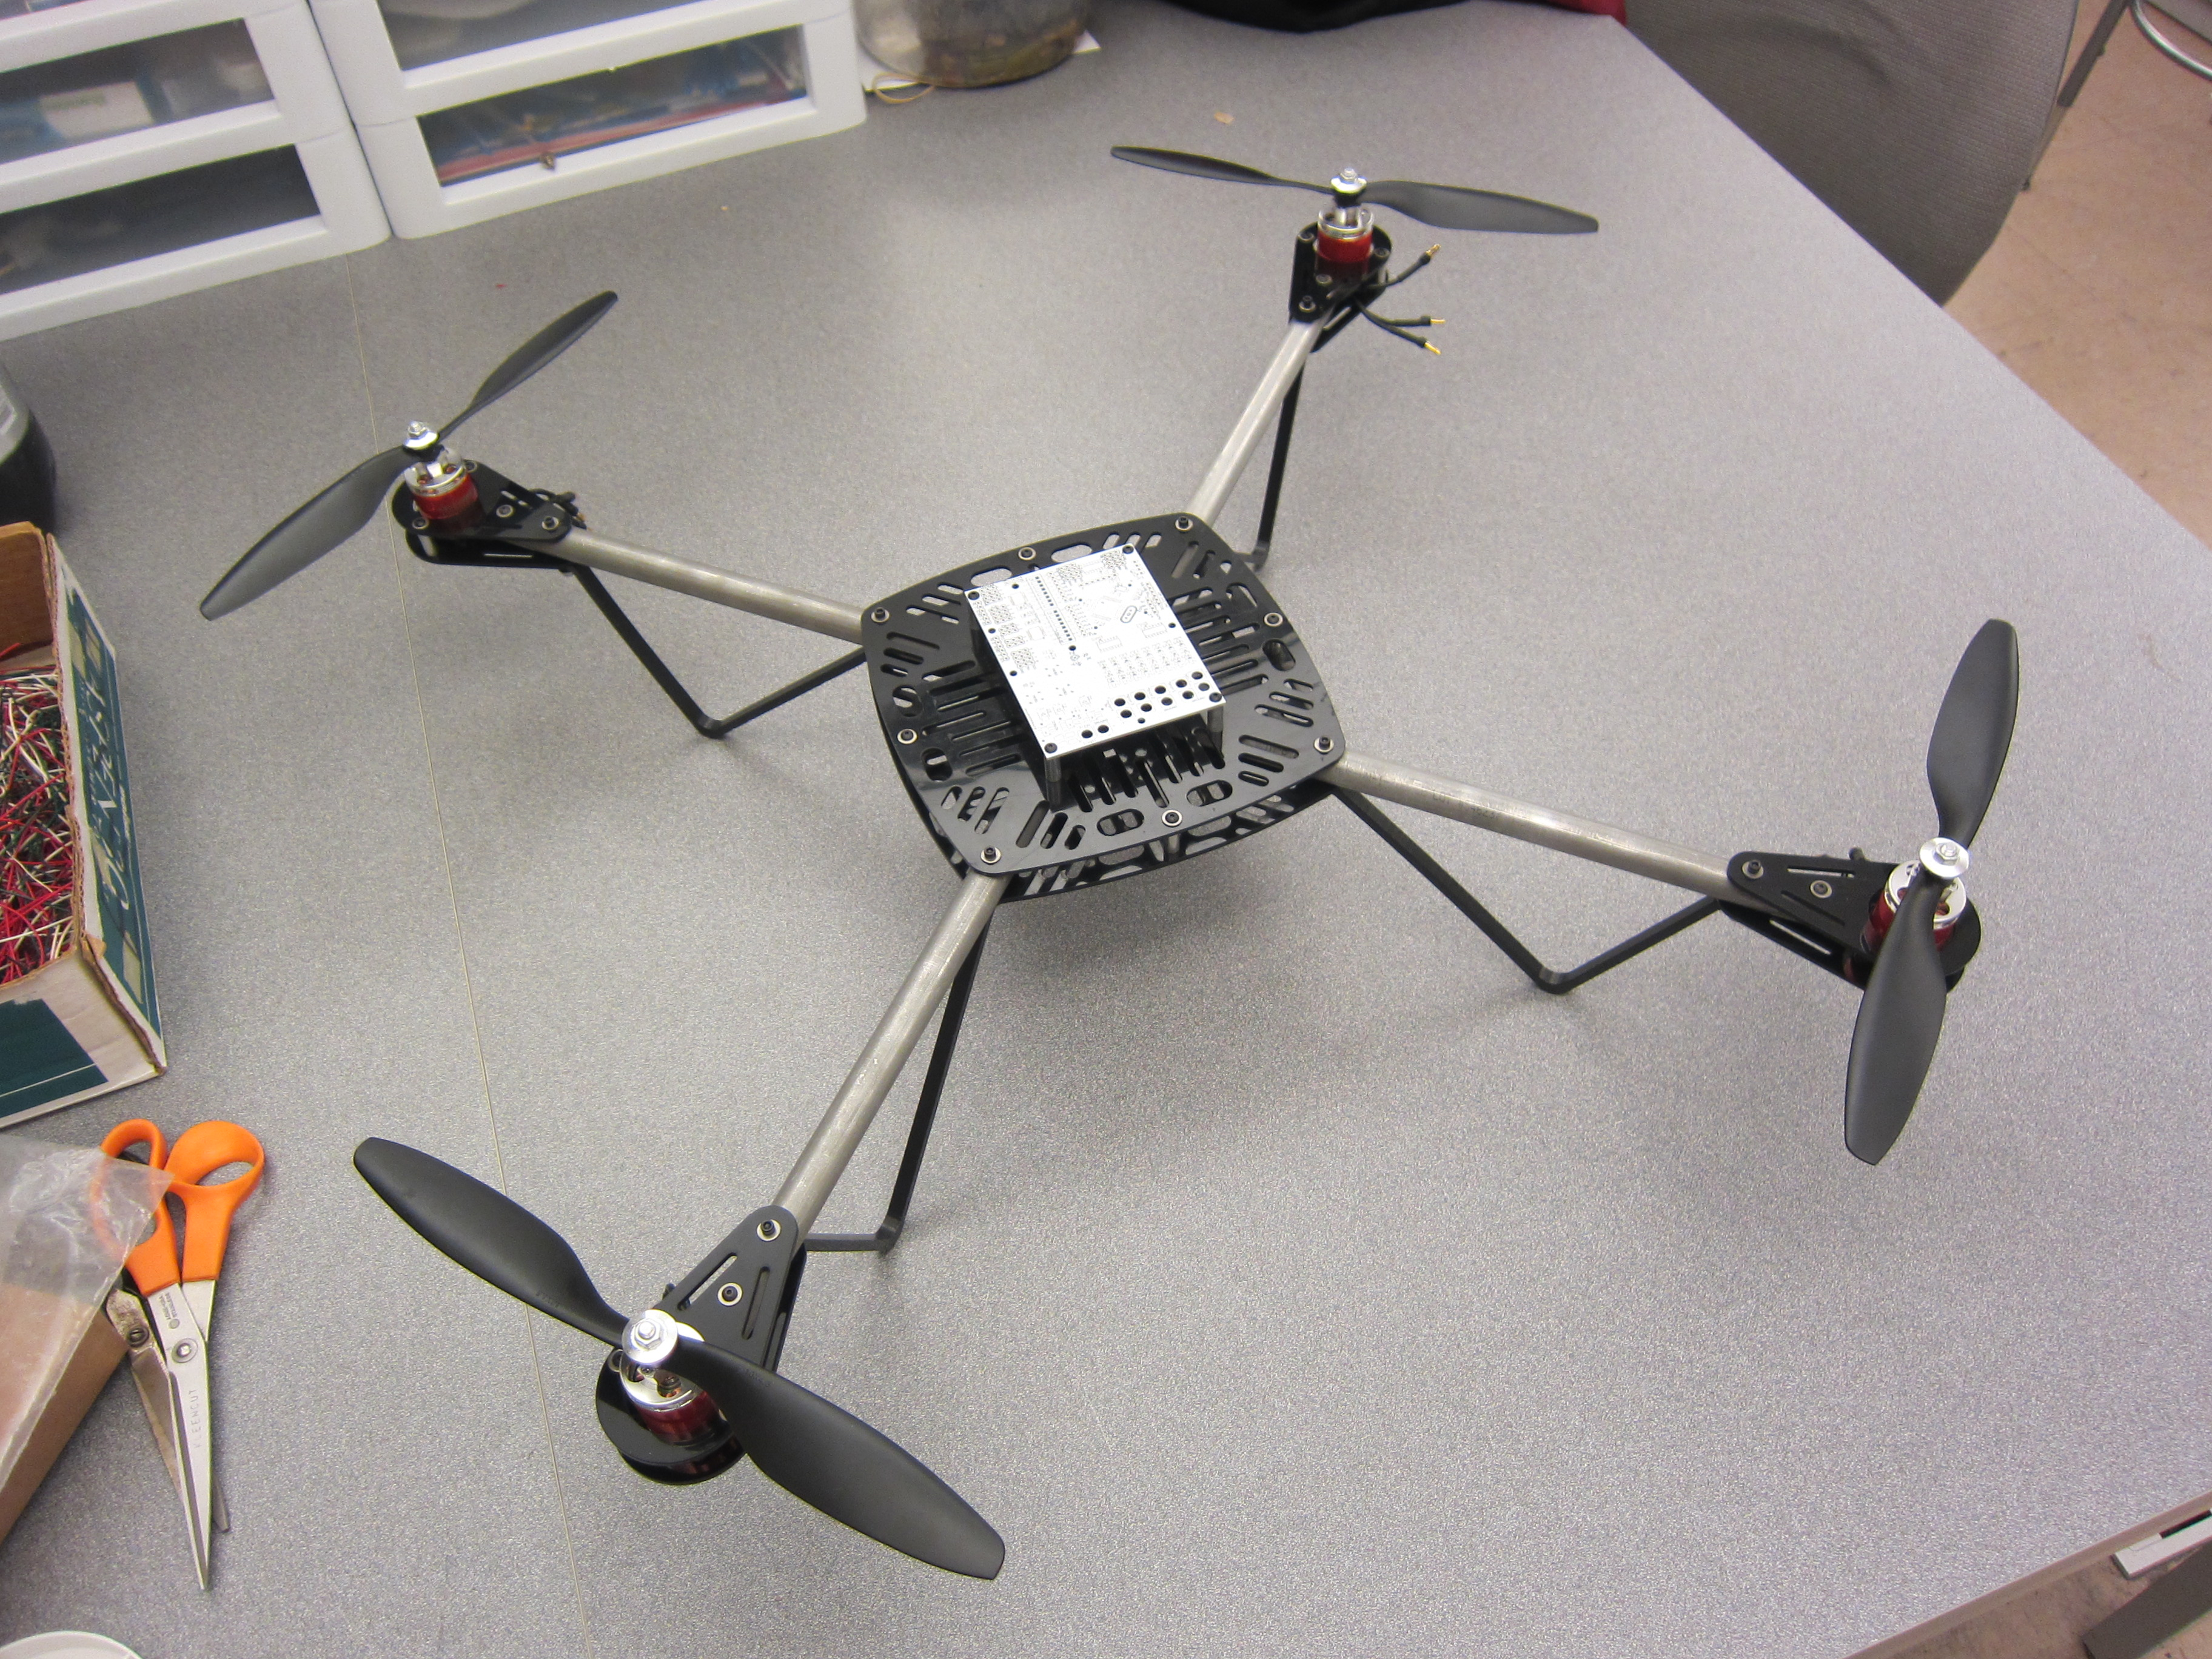
\includegraphics[scale=.07]{basic_quadrotor_platform.JPG}
  \caption{The Elev-8 quadrotor frame.}
\end{figure}  
  
  
This section describes all the equations necessary to have a stable hovering platform, and their order of implementation. It is broken down into three logical blocks: moment calculations (\ref{subsec:momentcalculations}), z axis force calculations (\ref{subsec:zaxisforcecalculations}), and motor speed calculations (\ref{subsec:motorspeedcalculations}). 
\\ \\
It is assumed that all math is done with floating point operations, and that the variables $t_i$ are temporary variables that can be used to hold a value for a short duration of time.


%% S2 S2 S2 S2 S2 S2 S2 S2 S2 S2 S2 S2 S2 S2 S2 S2 S2 S2 S2 S2  
\subsection{Thrust and Torque Coefficient Measurements} \label{subsec:thrustandtorquecoefficientmeasurements}
%% S2 S2 S2 S2 S2 S2 S2 S2 S2 S2 S2 S2 S2 S2 S2 S2 S2 S2 S2 S2  

In the equations to calculate the thrust (\ref{eq:motor_thrust}) and torque (\ref{eq:motor_torque}) of each motor we have two constants, $K_T$ and $K_Q$ that need to be measured empirically. The two equations are reproduced below:

\begin{equation} %\label{eq:motor_thrust}
K_T = \frac{T}{\rho n^2 D^4}
\end{equation}

\begin{equation} %\label{eq:motor_torque}
K_Q = \frac{Q}{\rho n^2 D^5}
\end{equation}
\\ \\
Our test stand must be able measure thrust, torque, rotational speed, rotor diameter, and air density.

%% S2 S2 S2 S2 S2 S2 S2 S2 S2 S2 S2 S2 S2 S2 S2 S2 S2 S2 S2 S2  
\subsection{Moment Calculations} \label{subsec:momentcalculations}
%% S2 S2 S2 S2 S2 S2 S2 S2 S2 S2 S2 S2 S2 S2 S2 S2 S2 S2 S2 S2  
This subsection calculates the moments $M_x$, $M_y$, and $M_z$ from the current orientation $\bs{q}$ and the desired orientation $\bs{q}_d$. The full derivation can be found in sections \ref{subsec:rollpitchyawerrors} and \ref{subsec:attitudestabilization}.


\bigskip

Input variables:
\begin{tabular}{l l}
 	$ \bs{\omega}_{b} $ 	& angular velocity in the body frame ($rad/s$) \\
 	$ \mathbf{q} $ 			& attitude quaternion \\
 	$ \mathbf{q}_d $		& desired quaternion \\
\end{tabular}

\bigskip

Input constants:
\begin{tabular}{l l}
 	$K_{PH} $				& tilt moment proportional constant \\
 	$K_{DH} $				& tilt moment derivative constant \\
 	$K_{Pz} $				& yaw moment proportional constant \\
 	$K_{Dz} $				& yaw moment derivative constant \\ 	
\end{tabular}

\bigskip

Output:
\begin{tabular}{l l}
	$ M_{x} - M_{z} $		& total rotor moments along each axis ($N \cdot m$) \\
\end{tabular}



{\allowdisplaybreaks \begin{align}
\tilde{\bs{q}} &= \bs{q}_d \otimes \bs{q}^* \\%eq:errorquaternion}
\alpha &= 2\arccos{\left(\tilde{q_0}\right)} \\%eq:errorquaternionalpha}
t_1 &= \sin{\alpha/2} \\
\bs{r}_{e_1} &= \frac{\tilde{q_1}}{t_1} \\
\bs{r}_{e_2} &= \frac{\tilde{q_2}}{t_1} \\
\bs{r}_{e_3} &= \frac{\tilde{q_3}}{t_1} \\
\bs{r}_b &= \bs{q}^* \otimes \bs{r}_e \otimes \bs{q} \\
\tilde{\bs{q}}_b &= 
\begin{bmatrix}
	\cos \left( \alpha / 2 \right) \\
	\sin \left( \alpha / 2 \right) \cdot \bs{r}_b
\end{bmatrix} \\
	\alpha_H &= \arccos \left[1 - 2 \left( q_1^2 + q_2^2 \right) \right] \\
	\psi &= 2 \arctan_2 \left( q_3, q_0 \right) \\
	t_1 &= \cos \left( \psi / 2 \right) \\
	t_2 &= \sin \left( \psi / 2 \right) \\
	t_3 &= \sin \left( \alpha_H / 2 \right) \\
	r_x &=   \frac{ t_1 q_1 - t_2 q_2}{ t_3} \\
	r_y &=   \frac{t_2 q_1 - t_1 q_2} { t_3 }  \\
	\beta_H &= \arctan_2 \left(r_y, r_x \right) \\
	M_x &= K_{PH} \alpha_H \cos \beta_H - K_{DH} \omega_x \\
	M_y &= K_{PH} \alpha_H \sin \beta_H - K_{DH} \omega_y \\
	M_z &= K_{Pz} \psi - K_{Dz} \omega_z
\end{align}}


%% S2 S2 S2 S2 S2 S2 S2 S2 S2 S2 S2 S2 S2 S2 S2 S2 S2 S2 S2 S2  
\subsection{Z Axis Force Calculations} \label{subsec:zaxisforcecalculations}
%% S2 S2 S2 S2 S2 S2 S2 S2 S2 S2 S2 S2 S2 S2 S2 S2 S2 S2 S2 S2  
This subsection calculates the necessary total thrust along the quadrotor z axis. This section takes the desired altitude and the current orientation and outputs the resultant $F_z$ necessary. The relevant equation derivations can be found in section \ref{subsec:altitudestabilization}.

\bigskip
Input variables:
\begin{tabular}{l l}
 	$ \mathbf{q} $ 			& attitude quaternion \\
 	$ \boldsymbol{R}_{e_z} $	& position in the inertial frame ($m$) \\
 	$ F_{z} $				& total force of the rotors on the z axis ($N$) \\
 	$desired \left( \bs{R}_{e_z} \right)$ & Desired z position (altitude) (m) \\
\end{tabular}

\bigskip
Input Constants:
\begin{tabular}{l l}

 	$m$						& quadrotor mass ($kg$ ?) \\
 	$g$						& local gravity ($m/s^2$) \\
 	$K_{P_z}$				& Proportional PID gain for $F_z$ \\
	$K_{I_z}$				& Integral PID gain for $F_z$ \\
	$K_{I_z}$				& Derivative PID gain for $F_z$ \\
\end{tabular}

\bigskip
Output Variables:
\begin{tabular}{l l}
 	$ F_{z} $				& total force of the rotors on the z axis ($N$) \\
\end{tabular}




\begin{align}
K_{tilt} &= 
	\begin{bmatrix}
		0 & 0 & 1 \\	
	\end{bmatrix}
	\cdot
	\left(
		q \otimes
			\begin{bmatrix}
				0 \\
				0 \\
				-1 \\
			\end{bmatrix}
		\otimes q^*
	\right) \\
\tilde{\bs{R}}_{e_z} &= \bs{R}_{e_z} - desired \left( \bs{R}_{e_z} \right) \\
	F_{PIDz} &= K_{Pz} \tilde{\bs{R}}_{e_z} + K_{Iz} \Sigma \tilde{\bs{R}}_{e_z} + K_{Dz} \dot{\tilde{\bs{R}}}_{e_z} \\ %\label{eq:altitudePID}
	F_z &= \frac{mg + F_{PIDz}} {K_{tilt}}
\end{align}





\clearpage

%% S2 S2 S2 S2 S2 S2 S2 S2 S2 S2 S2 S2 S2 S2 S2 S2 S2 S2 S2 S2  
\subsection{Motor Speed Calculations} \label{subsec:motorspeedcalculations}
%% S2 S2 S2 S2 S2 S2 S2 S2 S2 S2 S2 S2 S2 S2 S2 S2 S2 S2 S2 S2  
This subsection calculates the output command (i.e. motor speed) for each of the motors. The derivations for these equations can be found in sections \ref{subsec:forcestomotorspeeds} and \ref{subsec:motorcontrol}.

\bigskip
Input variables:
\begin{tabular}{l l}
 	$ F_{z} $				& total force of the rotors on the z axis ($N$) \\
 	$ M_{x}$, $M_y$, $M_{z} $		& total rotor moments along each axis ($N \cdot m$) \\
 	$ n_{imeas} $					& rotation frequency of the rotors ($Hz$) \\
 	%$ \Omega_i $			& rotation speed of the rotors ($rad / s$) \\	
 	%$ \Omega_{imeas} $		& measured rotation speed of the rotors ($rad / s$) \\

\end{tabular}

\bigskip
Input Constants:
\begin{tabular}{l l}
 	$ D $ 					& rotor diameter ($m$) \\
 	$ d $					& offset of each rotor from the center of mass ($m$) \\
 	$ \rho $				& air density ($kg/m^3$) \\
 	$ K_t $					& thrust coefficient \\
 	$ K_q $					& torque coefficient \\
 	$ K_{P_i} $				& Motor Proportional PID gain (for $1 \leq i \leq 4$) \\
 	$ K_{I_i} $				& Motor Integral PID gain (for $1 \leq i \leq 4$) \\
 	$ \pi $					& pi \\
\end{tabular}

\bigskip
Output Variables:
\begin{tabular}{l l}
 	$ u_i $					& motor command \\
\end{tabular}

%T &= K_T\rho n^2 D^4 \\ %\label{eq:motor_thrust}
%Q &= K_Q\rho n^2 D^5 \\ %\label{eq:motor_torque}

{\allowdisplaybreaks \begin{align} 
c &= \frac{K_Q D}{K_T} \\
t_1 &= \frac{M_z}{4c} \\
t_2 &= \frac{M_y}{2d} \\
t_3 &= \frac{M_x}{2d} \\
t_4 &= \frac{F_z}{4} \\
F_1 &= +t_1 - t_2 + t_4 \\
F_2 &= -t_1 - t_3 + t_4 \\
F_3 &= +t_1 + t_2 + t_4 \\
F_4 &= -t_1 + t_3 + t_4 \\
t_1 &= \frac{2 \pi}{D^2} \\
t_2 &= \rho K_T \\
\Omega_{d1}	&=  t_1 \sqrt{F_1 / t_2} \\% \label{eq:thrust_to_Omega}
\Omega_{d2}	&=  t_1 \sqrt{F_2 / t_2} \\% \label{eq:thrust_to_Omega}
\Omega_{d3}	&=  t_1 \sqrt{F_3 / t_2} \\% \label{eq:thrust_to_Omega}
\Omega_{d4}	&=  t_1 \sqrt{F_4 / t_2} \\% \label{eq:thrust_to_Omega}
\Omega \left(t \right)_{ Ierror1} &= \Omega \left(t-1 \right)_{ Ierror1} + \left( \Omega_{d1} - \Omega_{i1} \right) \\
\Omega \left(t \right)_{ Ierror2} &= \Omega \left(t-1 \right)_{ Ierror2} + \left( \Omega_{d2} - \Omega_{i2} \right) \\
\Omega \left(t \right)_{ Ierror3} &= \Omega \left(t-1 \right)_{ Ierror3} + \left( \Omega_{d3} - \Omega_{i3} \right) \\
\Omega \left(t \right)_{ Ierror4} &= \Omega \left(t-1 \right)_{ Ierror4} + \left( \Omega_{d4} - \Omega_{i4} \right) \\
u_1 &= K_{P1} \left( \Omega_{d1} - \Omega_{i1} \right) + K_{I1} \Omega \left(t \right) _{Ierror1} \\
u_2 &= K_{P2} \left( \Omega_{d2} - \Omega_{i2} \right) + K_{I2} \Omega \left(t \right) _{Ierror2} \\
u_3 &= K_{P3} \left( \Omega_{d3} - \Omega_{i3} \right) + K_{I3} \Omega \left(t \right) _{Ierror3} \\
u_4 &= K_{P4} \left( \Omega_{d4} - \Omega_{i4} \right) + K_{I4} \Omega \left(t \right) _{Ierror4}
\end{align}}
\\ \\
From here, we are able to send the command $u_i$ to the motor ESCs via a standard PWM signal. Note that the $u_i$ will have to be adjusted to fit within the standard servo type PWM signal standard. Typically, this means that the signal is set so that a motor speed of 0 corresponds to 1000uS, and a full motor speed corresponds to 2000uS, with a pulse every 20mS (approximately).













%% S1 S1 S1 S1 S1 S1 S1 S1 S1 S1 S1 S1 S1 S1 S1 S1 S1 S1 S1 S1  
\section{Basic Equations from \cite{stingu09}}
%% S1 S1 S1 S1 S1 S1 S1 S1 S1 S1 S1 S1 S1 S1 S1 S1 S1 S1 S1 S1  

The follow equations are exactly as written in \cite{stingu09}. The equations in previous sections follow the general guidelines of these equations, but some exceptions were made. They are here for reference only.

%% S2 S2 S2 S2 S2 S2 S2 S2 S2 S2 S2 S2 S2 S2 S2 S2 S2 S2 S2 S2  
\subsection{Quadrotor Model}
%% S2 S2 S2 S2 S2 S2 S2 S2 S2 S2 S2 S2 S2 S2 S2 S2 S2 S2 S2 S2  

\begin{equation}
\dot{\boldsymbol{V}}_b = \frac{1}{m} 
	\left[
		\begin{array}{c}
			0 \\
			0 \\
			F_z \\
		\end{array}
	\right]
	+ \boldsymbol{q}^* \otimes
		\left[
			\begin{array}{c}
				0 \\
				0 \\
				g \\
			\end{array}
		\right]
	\otimes \boldsymbol{q} - \boldsymbol{\omega}_b \times \boldsymbol{V}_b
\end{equation}

\begin{equation}
\dot{\boldsymbol{\omega}}_b = \boldsymbol{I}^{-1}_{nb}
	\left(
		\left[
			\begin{array}{c}
				M_x \\
				M_y \\
				M_z \\
			\end{array}
		\right]
		- \boldsymbol{\omega_b} \times \left( \boldsymbol{I}_{nb} \boldsymbol{\omega}_b \right)
	\right)
\end{equation}

\begin{equation}
\dot{\boldsymbol{R}}_e = \boldsymbol{q} \otimes \boldsymbol{V}_b \otimes \boldsymbol{q}^*
\end{equation}

\begin{equation}
\dot{\boldsymbol{q}} = \frac{1}{2} \boldsymbol{q} \otimes \boldsymbol{\omega}_b
\end{equation}

\begin{equation}
K_T = \frac{T}{\rho n^2 D^4}
\end{equation}

\begin{equation}
K_Q = \frac{Q}{\rho n^2 D^5}
\end{equation}

\begin{equation}
\Omega_i = 2 \pi n_i
\end{equation}

\begin{equation}
\tau \dot{\Omega}_i + \Omega_i = a_i f_{mot} \left(u_i, V_{batt} \right)
\end{equation}

\begin{equation}
\begin{bmatrix}
	F_z \\
	M_x \\
	M_y \\
	M_z \\
\end{bmatrix}
=
\begin{bmatrix}
	1 & 1 & 1 & 1 \\
	0 &-d & 0 & d \\
   -d & 0 & d & 0 \\
	c &-c & c &-c \\
\end{bmatrix}
\cdot
\begin{bmatrix}
	F_1 \\
	F_2 \\
	F_3 \\
	F_4 \\
\end{bmatrix}
\end{equation}
where
\begin{equation}
c = \frac{K_Q D}{K_T}
\end{equation}

\begin{equation}
\Omega_{di}=\frac{2 \pi}{D^2} \sqrt{ \frac{-F_{di}}{K_T \rho}}
\end{equation}

\begin{equation}
u_i = f_{mot}^{-1} \left( \frac{1}{a_i} \Omega_{di}, V_{batt} \right)
\end{equation}

%% S2 S2 S2 S2 S2 S2 S2 S2 S2 S2 S2 S2 S2 S2 S2 S2 S2 S2 S2 S2  
\subsection{Motor Gain Estimation}
%% S2 S2 S2 S2 S2 S2 S2 S2 S2 S2 S2 S2 S2 S2 S2 S2 S2 S2 S2 S2  

\begin{equation}
\dot{a}_i = K_g \left( \Omega_{imeas} - \hat{\Omega}_i \right)
\end{equation}

%% S2 S2 S2 S2 S2 S2 S2 S2 S2 S2 S2 S2 S2 S2 S2 S2 S2 S2 S2 S2  
\subsection{Yaw and Tilt Errors}
%% S2 S2 S2 S2 S2 S2 S2 S2 S2 S2 S2 S2 S2 S2 S2 S2 S2 S2 S2 S2  

\begin{eqnarray}
\bs{q}_d = \tilde{\bs{q}} \otimes \bs{q} \\
\tilde{\bs{q}} = \bs{q}_d \otimes \bs{q}^*
\end{eqnarray}

\begin{equation}
\tilde{\bs{q}} = 
\begin{bmatrix}
	\cos \left( \alpha / 2 \right) \\
	\sin \left( \alpha / 2 \right) \cdot \bs{r}_e
\end{bmatrix}
\end{equation}

\begin{equation}
\bs{r}_b = q^* \otimes \bs{r}_e \otimes \bs{q}
\end{equation}

\begin{equation}
\tilde{\bs{q}}_b = 
\begin{bmatrix}
	\cos \left( \alpha / 2 \right) \\
	\sin \left( \alpha / 2 \right) \cdot \bs{r}_b
\end{bmatrix}
\end{equation}

\begin{equation}
\tilde{\bs{q}}_b = \bs{q}_H \otimes \bs{q}_V
\end{equation}

\begin{equation}
	\begin{bmatrix}
		q_0 \\
		q_1 \\
		q_2 \\
		q_3 \\
	\end{bmatrix}
	=
	\begin{bmatrix}
		\cos \left( \alpha_H / 2 \right) \\
		\sin \left( \alpha_H / 2 \right) \cdot r_x \\
		\sin \left( \alpha_H / 2 \right) \cdot r_y \\
		\sin \left( \alpha_H / 2 \right) \cdot 0 \\
	\end{bmatrix}
	\otimes
	\begin{bmatrix}
		\cos \left( \psi / 2 \right) \\
		\sin \left( \psi / 2 \right) \cdot 0 \\
		\sin \left( \psi / 2 \right) \cdot 0 \\
		\sin \left( \psi / 2 \right) \cdot 1 \\
	\end{bmatrix}
\end{equation}

\begin{equation}
	\alpha_H = \arccos \left[1 - 2 \left( q_1^2 + q_2^2 \right) \right]	\qquad 0 \leq \alpha_H < \pi	
\end{equation}

\begin{equation}
	\psi = 2 \arctan_2 \left( q_3, q_0 \right) \qquad -\pi \leq \psi < \pi
\end{equation}

\begin{equation}
	r_x =   \frac{\cos \left( \psi / 2 \right) q_1 - \sin \left( \psi / 2 \right) q_2}
	{ \sin \left( \alpha_H / 2 \right) }
\end{equation}

\begin{equation}
	r_y =   \frac{\sin \left( \psi / 2 \right) q_1 - \cos \left( \psi / 2 \right) q_2}
	{ \sin \left( \alpha_H / 2 \right) }
\end{equation}

\begin{equation}
	\beta_H = \arctan_2 \left(r_y, r_x \right)
\end{equation}

\begin{equation}
	\gamma_H = \arctan_2 \left(r_x, r_y \right)
\end{equation}

%% S2 S2 S2 S2 S2 S2 S2 S2 S2 S2 S2 S2 S2 S2 S2 S2 S2 S2 S2 S2  
\subsection{Attitude stabilization}
%% S2 S2 S2 S2 S2 S2 S2 S2 S2 S2 S2 S2 S2 S2 S2 S2 S2 S2 S2 S2  

\begin{align}
	M_x &= K_{PH} \alpha_H \cos \beta_H - K_{DH} \omega_x \\
	M_y &= K_{PH} \alpha_H \sin \beta_H - K_{DH} \omega_y \\
	M_z &= K_{Pz} \psi - K_{Dz} \omega_z \\
\end{align}

%% S2 S2 S2 S2 S2 S2 S2 S2 S2 S2 S2 S2 S2 S2 S2 S2 S2 S2 S2 S2  
\subsection{Altitude Control}
%% S2 S2 S2 S2 S2 S2 S2 S2 S2 S2 S2 S2 S2 S2 S2 S2 S2 S2 S2 S2  

\begin{equation}
	F_z = \frac{mg + F_{PIDz}} {K_{tilt}}
\end{equation}

\begin{equation}
	K_{tilt} = 
	\begin{bmatrix}
		0 & 0 & 1 \\	
	\end{bmatrix}
	\cdot
	\left(
		q \otimes
			\begin{bmatrix}
				0 \\
				0 \\
				-1 \\
			\end{bmatrix}
		\otimes q^*
	\right)
\end{equation}







%To make really long equations:
%\begin{eqnarray*}
%  \lefteqn{\left(1+x\right)^n = } \\
%  & & 1 + nx + \frac{n\left(n-1\right)}{2!}x^2 + \\
%  & & \frac{n\left(n-1\right)\left(n-2\right)}{3!}x^3 + \\
%  & & \frac{n\left(n-1\right)\left(n-2\right)\left(n-3\right)}{4!}x^4 + \\
%  & & \ldots
%\end{eqnarray*}
%
%\section{Stuff I still need to address}
%\begin{list}{*}{}
%	\item Add tables with acronyms, abbreviations, and units
%	\item Add information on how to calculate moment of inertia tensor (make note of parallel axes theorem)
%	\item I made a note of "Origin at CoM, axes of inertia". What does it mean?
%	\item What is static / dynamic range (tracking)? In reference to yaw/roll/pitch error
%	\item Discuss kinematics vs. Dynamics
%	\item Add the derivation from brushless DC motor to brushed DC motor, specifically for thrust/torque
%	\item Add information about calculating "linear regression" to calculate motor constants from test data.
%	\item Add step by step information for testing thrust/torque
%	\item Check: when rolling/pitching/yawing, do these equations hold only for small differences in rotor speed? (source: the masters paper from Asia...)
%	\item I'm told that since the big matrix only has four possible inputs (4 motors), we can only control four things. But what about hex/octo rotors?
%	\item What about motor saturation? Should priority be given to attitude over altitude?
%	\item From the motor control section, "Does the system take into account that these are rotations, so that several values can represent the same rotation? eg $3\pi$ and $-\pi$.
%	\item Add a PID tutorial (how to prevent integral wind up; derivative impulse (that saturates))
%	\item I suspect that the $K_{tilt}$ equation can be simplified by taking the dot product of the two vectors, which (according to a UCSD slide show) is $p_0 q_0 +p_1 q_1 + p_2 q_2 + p_3 q_3 = |p||q| \cos \varphi$ where $\varphi$ is half the angle angle one would need to rotate from one orientation to the other in 3D space.
%	\item Add more information about the motor thrust test stand (subsection \ref{subsec:thrustandtorquecoefficientmeasurements})
%	\item Add citation for the quaternion norm debate (to square root or not).
%	\item Question: Order of the quaternion component multiplication doesn't matter, right? Also, double check the correct multiplication...
%	\item Equations \eqref{eq:motor_thrust} and \eqref{eq:motor_torque} are derived from --WHAT???.
%	\item Talk about quaternion derivatives, and equation \eqref{eq:omega_b_derivative}
%	\item Quantify by how much performance will suffer if air density is assumed to be constant.
%	\item Should this subsection (\ref{subsec:motorspeedcalculations}) have something in here where it converts $n_i$ to $omega_i$? Ie, from RPM to rad/s?
%	\item Should this subsection (\ref{subsec:motorspeedcalculations}) have something in the PID where it uses the measured speed of the propellers?
%	\item  Is $q^*$ the correct notation for conjugate?
%	\item Is it a conversion between RPM and Rad/S in section \ref{subsec:forcestomotorspeeds}?
%
%
%\end{list}
%
%Specifically, with quaternions:
%---Need to define the fact that two quaternions can represent the same space \\
%---Need to define quaternion derivatives --- \\
%---What is $q^*$?--- \\
%


\begin{thebibliography}{99}

%Use postfix of 69 to indicate unknown year

	\bibitem{stingu09}
	E. Stingu, F. Lewis, 
	"Design and Implementation of a Structured Flight Controller for a 6DoF Quadrotor Using Quaternions," 
Mediterranean Conference on Control \& Automation, pp. 1233-1238, June 2009.


	% Justifies the use of a square root in quaternion norm
	\bibitem{malek09} % www.mcs.csueastbay.edu/~malek/Class/norm.pdf
	M. Malek,
	"Vector and Matrix Norms", California State University, East Bay, May 2009.
	
	\bibitem{shoemake69} % www.cs.ucr.edu/~vbz/resources/quatut.pdf
	K. Shoemake,
	"Quaternions", Department of Computer and Information Science, University of Pennsylvania.
	
	
	
\end{thebibliography}

\end{document}

















